\subsection{Hormiga de Langton}

El último experimento de esta sección busca imitar el comportamiento de la hormiga de Langton, un agente reactivo que vive en un espacio bidimensional. Este sistema no fue concebido como un autómata celular en un sentido estricto, pero a diferencia de \textit{sandpile}, sí se puede definir como uno sin necesidad de manipular su comportamiento. 

Originalmente, la hormiga de Langton realiza un par de acciones según el estado de la célula que esté pisando, estas incluyen cambiar el color y cambiar de dirección. La representación mediante un autómata celular pone el foco en cada célula, donde la mayoría está en un estado de naturaleza muerta hasta que tienen un vecino que contiene una hormiga a punto de caminar encima de ella.

Para este experimento se considera la convención original en una cuadrícula, cada una con 2 estados y una hormiga con 2 instrucciones, girar a la derecha con blancos y a la izquierda con negros. Además, para representar la posición de la hormiga se requieren dos conjuntos de estados que incluyen las cuatro direcciones para blanco y negro. 

Es necesario considerar la dirección por cada color. Considerando la célula del centro en el siguiente escenario:
\[
\left[
\begin{matrix}
	0 & \downarrow & 0 \\
	0 & 0 & 0 \\
	0 & 0 & 0 
\end{matrix} \right] \rightarrow
\left[ \begin{matrix}
	0 & 0 & 0 \\
	0 & \leftarrow & 0 \\
	0 & 0& 0 \\
\end{matrix}  \right]\rightarrow
\left[ \begin{matrix}
0 & 0 & 0 \\
\uparrow & x & 0 \\
0 & 0& 0 \\
\end{matrix}  \right]
\]
En el primer paso, la información que recibe de sus vecinos y de sí misma es que una hormiga caminará sobre él y cambiará su dirección. En el siguiente paso, sabe que tiene que dejar de ser una hormiga y convertirse en un estado, pero el sistema no tiene memoria, es decir, no recuerda qué estado era antes de ser la dirección de la hormiga, por lo que pierde el contexto de la situación.

El vector de regla tiene un tamaño de $10^{5} = 100{,}000$, y la hormiga de Langton es una regla entre $10^{100000}$. Otra limitación de este sistema es la cantidad de información que presenta, pues los únicos cambios existen cuando una hormiga está cerca. Tratar a la hormiga como un autómata celular es computacionalmente más complejo, pero este experimento busca la extracción de sistemas con poca información. 

En un espacio de $100 \times 100$ si evolucionamos el sistema por 11,000 pasos con una configuración inicial vacía obtenemos la distribución de estados de la figura \ref{fig:langton_RL_100x100_proporcion}, donde se observa el problema de distribución de clases. Por otro lado, si consideramos múltiples condiciones iniciales aleatorias pero una única hormiga, obtenemos los datos de la figura \ref{fig:langton_RL_aleatorias_proporcion}, donde la única diferencia es la distribución entre ceros y unos. 

\begin{figure}[htbp]
	\centering
	\begin{subfigure}[b]{0.45\textwidth}
		\centering
		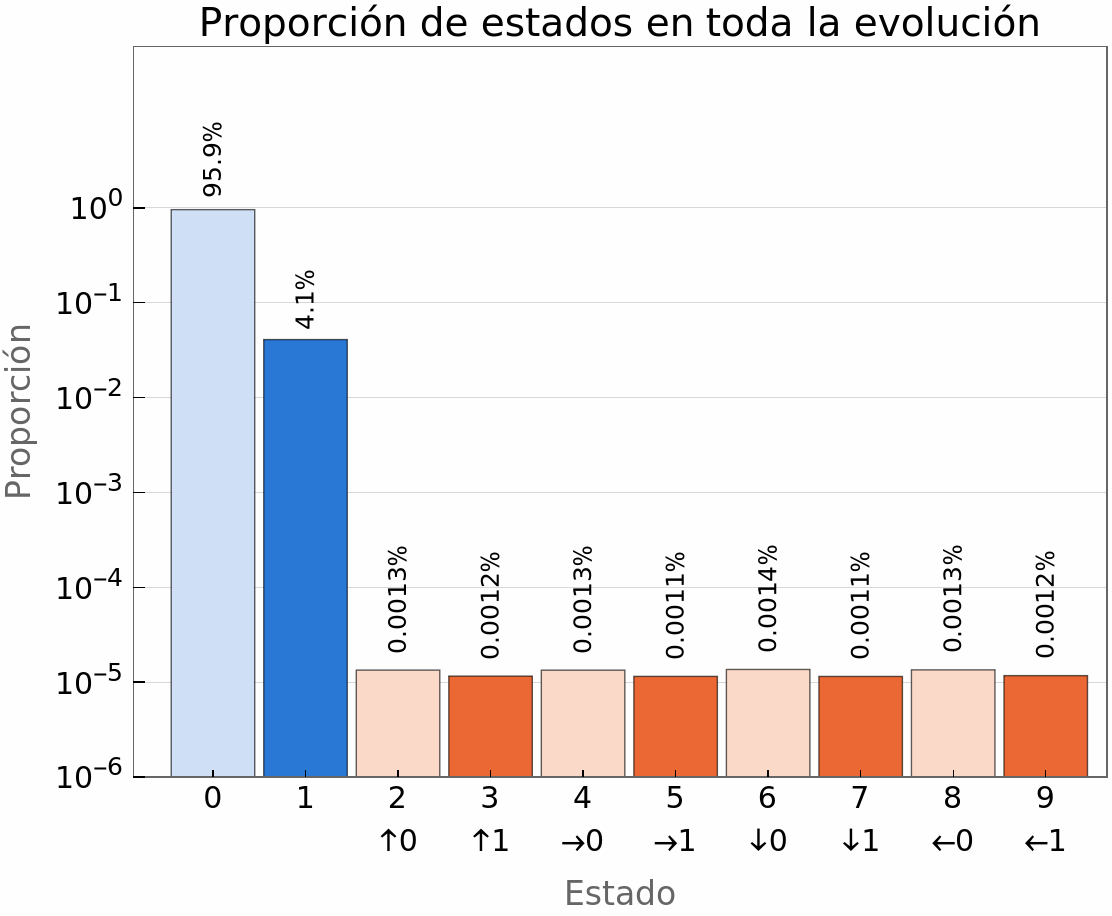
\includegraphics[width=0.9\linewidth]{img/experimentacion/duplicacion/langton/langton_RL_100x100_proporcion.png}
		\caption{11000 pasos con una configuración inicial vacía. }
		\label{fig:langton_RL_100x100_proporcion}
	\end{subfigure}
	\hfill 
	\begin{subfigure}[b]{0.45\textwidth}
		\centering
		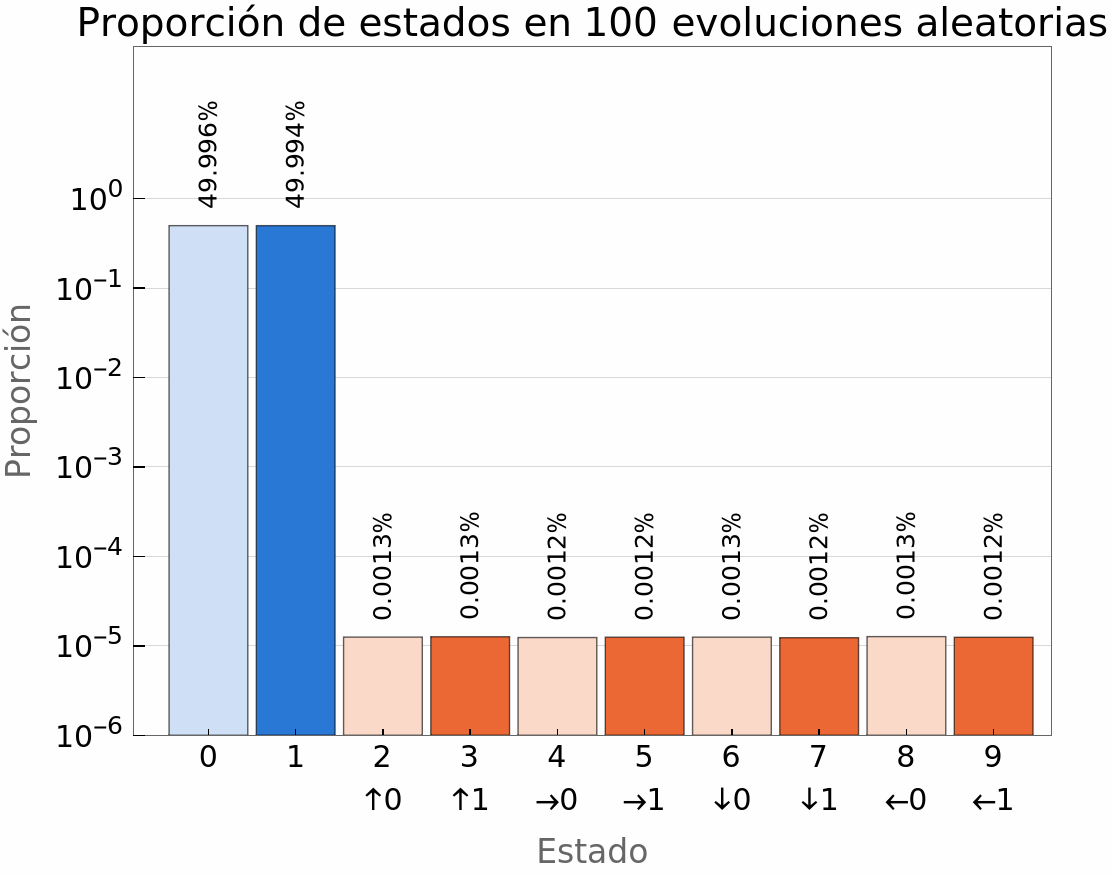
\includegraphics[width=0.9\linewidth]{img/experimentacion/duplicacion/langton/langton_RL_aleatorias_proporcion.png}
		\caption{100 pruebas durante 1,000 pasos con configuraciones iniciales aleatorias.}
		\label{fig:langton_RL_aleatorias_proporcion}
	\end{subfigure}
	\caption{Distribuciones de probabilidad de los 10 estados de una hormiga de Langton RL. Escala logarítmica.}
	\label{fig:langton_distribucion}
\end{figure}

\subsubsection{Capacidad de replicación}

Con una red neuronal dada por 2:8:ReLU \& 10:Linear, una tasa de aprendizaje de 0.001 y una pérdida objetivo de 0.0001, el autómata celular neuronal pudo replicar el comportamiento de una hormiga en el espacio a la perfección en tan solo 36 épocas usando \textit{one-hot encoding}. En la figura \ref{fig:langton_RL_paso_11000} se muestra el paso 11,000 de la hormiga generado en Mathematica y por el autómata celular neuronal en el simulador, y su coincidencia en el mismo punto.

\begin{figure}[htbp]
	\centering
	\begin{subfigure}[b]{0.45\textwidth}
		\centering
		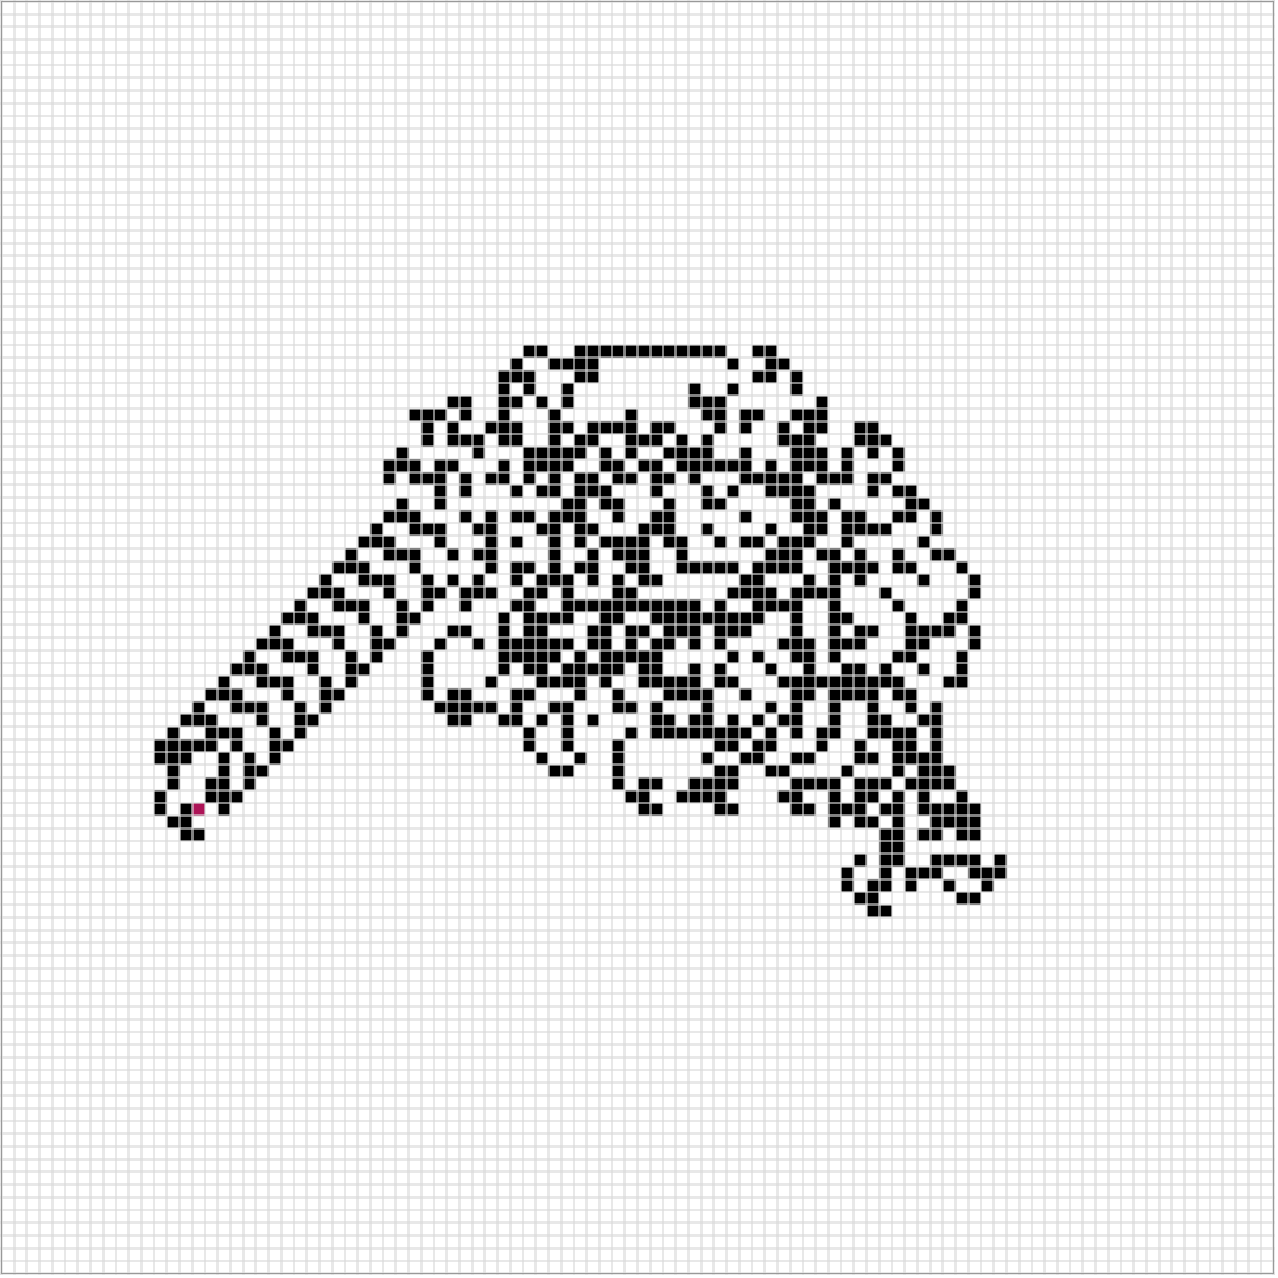
\includegraphics[width=0.7\linewidth]{img/experimentacion/duplicacion/langton/langton_RL_100x100_paso_11000.png}
		\caption{Evolución de la hormiga de Langton generada en Mathematica.}
		\label{fig:langton_RL_100x100_paso_11000}
	\end{subfigure}
	\hfill 
	\begin{subfigure}[b]{0.45\textwidth}
		\centering
		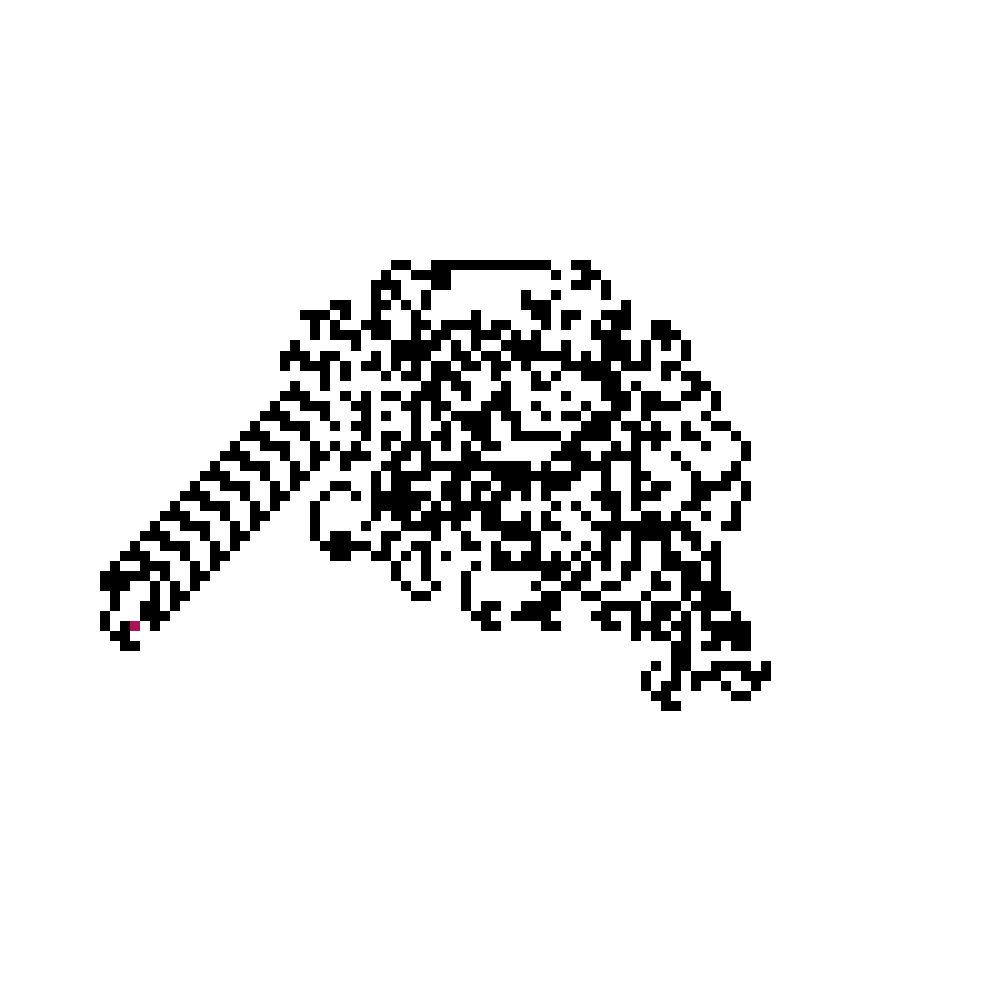
\includegraphics[width=0.67\linewidth]{img/experimentacion/duplicacion/langton/langton_RL_nca_100x100_paso_11000.png}
		\caption{Evolución del autómata celular neuronal originado en el simulador.}
		\label{fig:langton_RL_nca_100x100_paso_11000}
	\end{subfigure}
	\caption{Comparativa del agente Langton y el autómata celular neuronal entrenado después de 11,000 pasos con la misma configuración inicial. }
	\label{fig:langton_RL_paso_11000}
\end{figure}

\subsubsection{Colisión de múltiples hormigas}

Al colocar dos hormigas con la misma regla en el mismo espacio, su comportamiento suele ser independiente y ocurre sin errores hasta que se aproximan entre ellas. En la figura \ref{fig:langton_RL_nca_patrones_multi} se muestran los posibles patrones de dos hormigas donde una apunta a otra, en todos ellos, se realiza la sustitución correcta. El autómata celular neuronal extrapoló su conocimiento con una única hormiga para satisfacer estas condiciones. 

\begin{figure}[H]
	\centering
	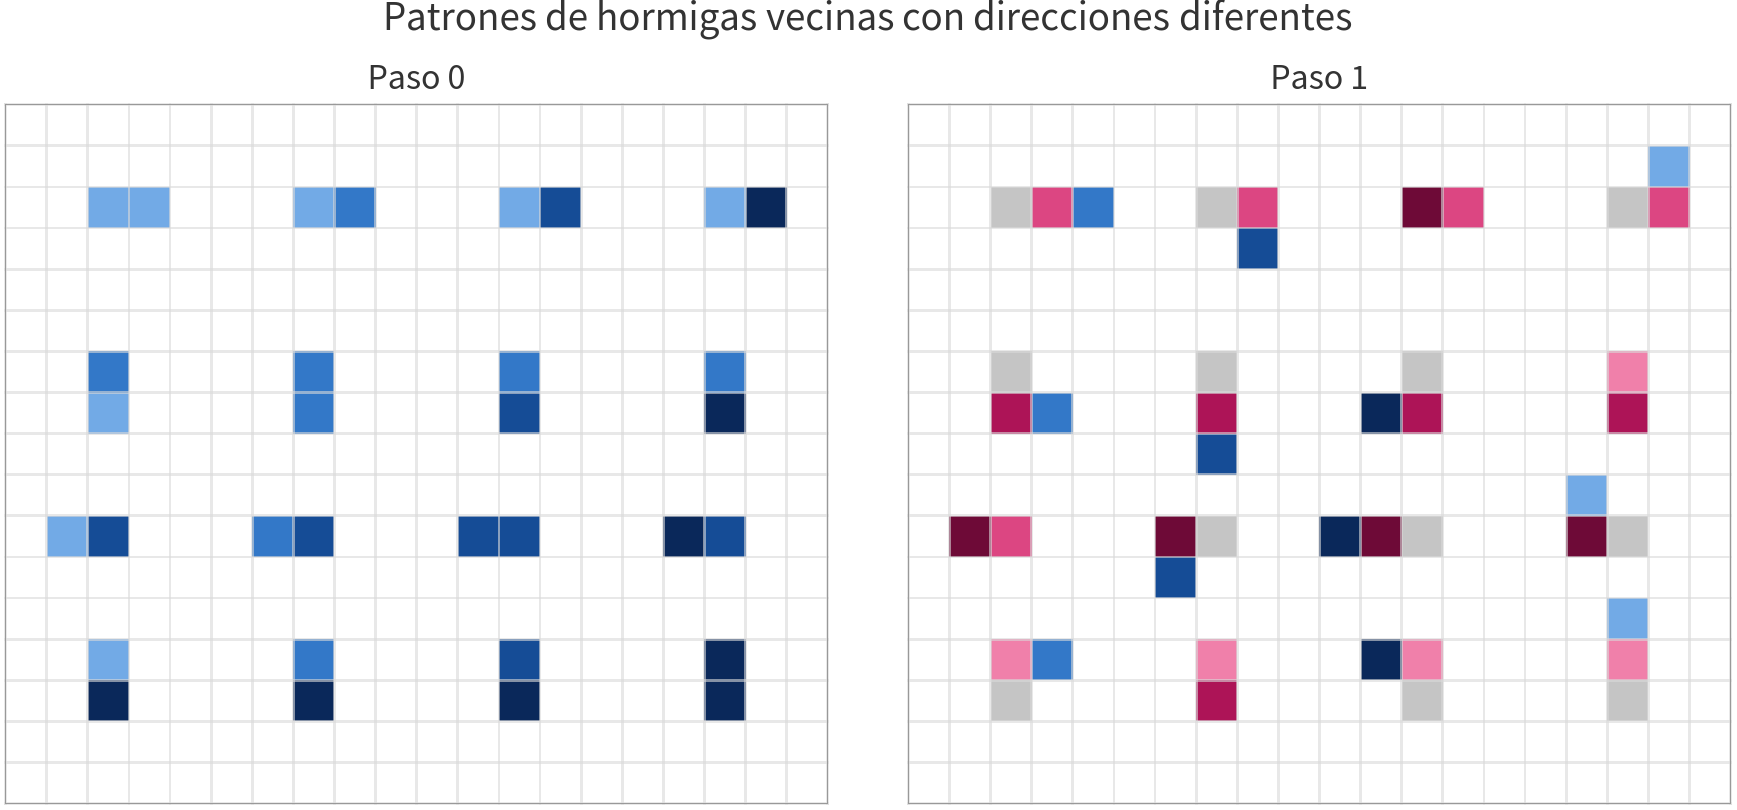
\includegraphics[width=0.5\linewidth]{img/experimentacion/duplicacion/langton/langton_RL_nca_patrones_multi.png}
	\caption{Preservación de hormigas vecinas bajo múltiples combinaciones.}
	\label{fig:langton_RL_nca_patrones_multi}
\end{figure}

Adicionalmente, en la figura \ref{fig:langton_RL_nca_patrones_combi} se muestran todos los patrones en donde dos hormigas colisionan en el siguiente paso. La solución que da el autómata celular neuronal es eliminar una de ellas.

\begin{figure}[H]
	\centering
	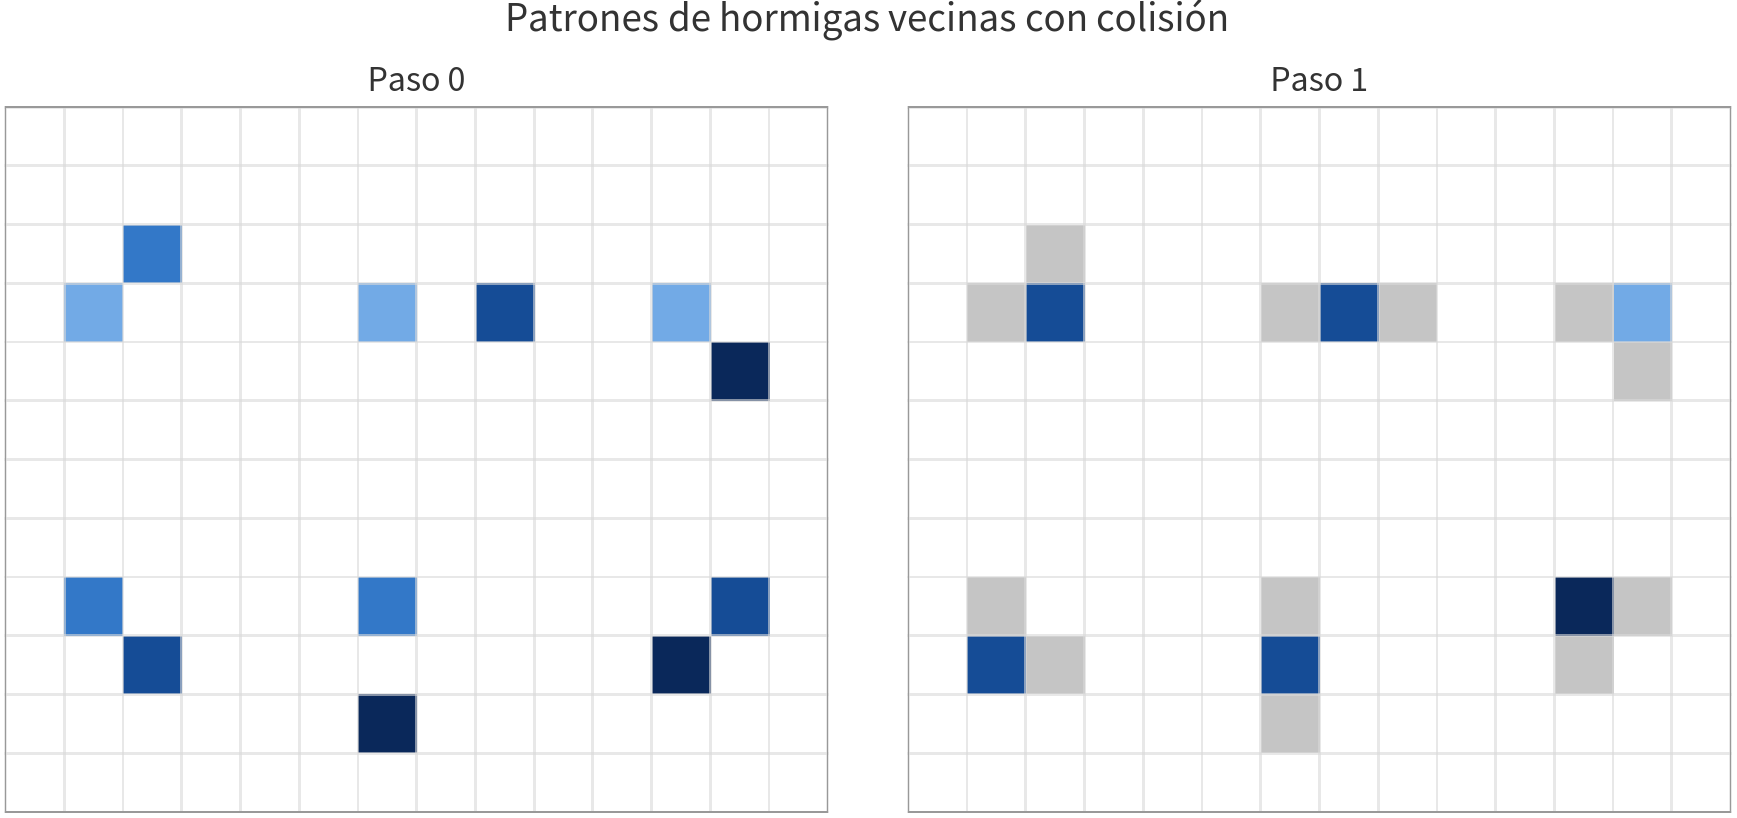
\includegraphics[width=0.5\linewidth]{img/experimentacion/duplicacion/langton/langton_RL_nca_patrones_combi.png}
	\caption{Eliminación de hormigas bajo múltiples combinaciones que colisionan en el paso 1.}
	\label{fig:langton_RL_nca_patrones_combi}
\end{figure}

Las simulaciones con múltiples hormigas deben tener una regla adicional que defina el comportamiento cuando hay colisiones, algunas opciones son:
\begin{itemize}
	\item Las hormigas son independientes: Cada hormiga ignora a las otras hormigas y solo le interesa el estado de la célula. Esta solución requiere incrementar el número de estados de manera proporcional al número de hormigas. Por lo que se requeriría definir el comportamiento de cuando hasta 4 hormigas colisionan en el mismo punto, situaciones menos probables que dependerían de preparar escenarios manuales para fomentar su aparición.
	\item Rotar sin avanzar: Es decir, si dos hormigas van a colisionar, se define una regla que ninguna ocupará ese espacio y en su lugar, cada una de ellas rota sobre su eje. Esta solución resuelve el problema, pero agrega un comportamiento adicional a la hormiga. 
	\item Actualización asíncrona: Las hormigas tienen un orden de prioridad, si se define se incrementa el número de estados, si no, rompe la definición de autómata celular.
	\item Combinación de hormigas: Solo una de ellas sobrevive cuando colisionan, resultado que fue inferido por el autómata celular neuronal.
\end{itemize}

Esta discrepancia se origina porque no existe una definición formal de cuál debe ser el comportamiento de múltiples hormigas en el mismo espacio, pues la idea fue concebida para una única hormiga.

\subsubsection{Crecimiento de estados}

Para finalizar, se explora el crecimiento del número de estados. La hormiga de Langton se generaliza a $n$ colores mediante una cadena de instrucciones, donde la letra $i$ indica el giro sobre una célula de color $i$ (R a la derecha, L a la izquierda), y la célula pasa al color $(i+1) \bmod n$. Con $n$ colores y cuatro direcciones, el autómata celular requiere $n + 4n = 5n$ estados, por lo que de 2 a 10 colores se pasa de 10 a 50 estados.

Para cada número de colores se generó un conjunto de datos con dos hormigas en un espacio de $30 \times 30$ con frontera periódica durante 10,000 pasos, usando la regla de rotar sin avanzar cuando dos hormigas van a colisionar. Para cada $n$ se eligió la regla que distribuye los colores de forma más uniforme, ignorando aquellas que repiten una más corta (por ejemplo, RRLRRL se comporta como RRL). La vecindad es un rombo de radio 2 (13 células), pues una célula necesita saber si otra hormiga a dos células de distancia también apunta hacia ella. Todas las redes tienen la forma 4:64:ReLU \& $5n$:Linear con \textit{one-hot encoding}, una tasa de aprendizaje inicial de 0.001 que se reduce a la mitad cuando la pérdida no mejora en 20 épocas, una pérdida objetivo de $1 \times 10^{-7}$ y semilla 42.

En la tabla \ref{tab:langton_colores} se observa que el número de estados casi no afecta el entrenamiento: todas las configuraciones alcanzaron la pérdida objetivo en menos de 90 épocas y menos de 100 segundos. Además, el número de épocas no crece de forma monótona con el número de colores. A partir de 8 colores la tasa de aprendizaje se redujo una vez, a 0.0005. Ocho de las nueve redes reproducen los 10,000 pasos de su evolución sin errores. La excepción es la regla RRRLLL (6 colores), que tiene un único error en 9 millones de células, en un paso donde las hormigas colisionan, lo que hace que la evolución diverja en el paso 7,028.

\begin{table}[H]
	\centering
	\begin{tabular}{c c l c c c}
		\toprule
		Colores & Estados & Regla & Épocas & Pérdida final & Tiempo \\
		\midrule
		2  & 10 & RL         & 22 & $5.18 \times 10^{-8}$ & 25.6 s \\
		3  & 15 & RLL        & 63 & $3.83 \times 10^{-8}$ & 73.8 s \\
		4  & 20 & RLLR       & 16 & $3.27 \times 10^{-8}$ & 20.0 s \\
		5  & 25 & RLRLL      & 44 & $7.81 \times 10^{-8}$ & 51.3 s \\
		6  & 30 & RRRLLL     & 68 & $4.35 \times 10^{-8}$ & 75.4 s \\
		7  & 35 & RLRLRLL    & 77 & $6.77 \times 10^{-9}$ & 85.7 s \\
		8  & 40 & RLRLRLRR   & 63 & $1.57 \times 10^{-8}$ & 70.4 s \\
		9  & 45 & RLRLRLLRL  & 63 & $2.31 \times 10^{-8}$ & 73.7 s \\
		10 & 50 & RLRLRLRRRL & 87 & $2.38 \times 10^{-9}$ & 97.3 s \\
		\bottomrule
	\end{tabular}
	\caption{Entrenamiento de la hormiga de Langton con dos hormigas de 2 a 10 colores. Espacio de $30 \times 30$, 10,000 pasos, red 4:64:ReLU \& $5n$:Linear con \textit{one-hot encoding}, pérdida objetivo $1 \times 10^{-7}$.}
	\label{tab:langton_colores}
\end{table}

Sin embargo, reproducir la evolución de entrenamiento no implica haber aprendido la regla. Con la regla de 10 colores, una única hormiga orientada hacia la izquierda, en el centro de un espacio de $100 \times 100$ con frontera periódica, evoluciona sin errores hasta el paso 12,455, donde la hormiga se divide en dos. La hormiga gira y avanza correctamente, pero la célula que deja no cambia de color y conserva una hormiga girada, como si hubiera estado bloqueada por otra. Es decir, el autómata celular neuronal aplica la regla de colisión aprendida de los datos con dos hormigas en un patrón que nunca vio durante el entrenamiento, aunque no haya otra hormiga cerca.

Con este último experimento observamos que el autómata celular neuronal puede reproducir comportamientos complejos con un número creciente de estados. El sistema tradicional pudo ser replicado con exactitud y, con hasta 10 colores (50 estados, $50^{13}$ patrones y $50^{50^{13}}$ reglas totales), las redes reprodujeron su evolución de entrenamiento, es decir, extrajeron la parte de la función de transición presente en esos datos. Sin embargo, fuera de ellos aparecen errores como la división de la hormiga, por lo que reproducir la evolución no garantiza haber extraído la función de transición en su totalidad.

Además, se pudo generalizar el comportamiento de una hacia dos hormigas cuando no colisionan pero sí son vecinas, comportamiento que no estuvo presente durante el entrenamiento. Finalmente, aplicó la eliminación de hormigas que, aunque pudo haber utilizado cualquier función para definir ese comportamiento, fue constante en todas las combinaciones donde colisionaban.

Esta serie de tres experimentos (juego de la vida, modelo de \textit{sandpile} y hormiga de Langton) ayudaron no solo a probar las capacidades de replicación de la red neuronal al momento de experimentar con sistemas complejos, sino que adicionalmente ayudaron a 
\begin{itemize}
	\item Definir la mejor estructura de la red neuronal: Se encontró que ReLU en las capas ocultas y Linear en la capa de salida suele tener los mejores resultados. Además, no es necesario tener redes muy profundas, en su lugar, es recomendado tener pocas capas con mayor número de neuronas cada una. 

	\item Seleccionar hiperparámetros: Comparando métodos de reducción de tasa de aprendizaje, se concluyó que una reducción dinámica es una opción viable cuando la pérdida empieza a tener un comportamiento oscilatorio. 

	\item Definir la capa de entrada: Esto mediante una codificación \textit{one-hot} que elimina la linealidad entre los datos y agiliza el entrenamiento de la red neuronal drásticamente. 
	
	\item Comprender la generalización de comportamientos: Cómo se adapta ante escenarios nunca antes vistos o muy poco frecuentes pero manteniendo su dinámica principal.
\end{itemize}

Estas tareas ayudaron a implementar mejoras dentro del simulador así como configurar el autómata celular neuronal para los próximos experimentos, en donde se busca imitar el comportamiento de sistemas complejos que se encuentren en la naturaleza.
